\section{Introduction}
\pagenumbering{arabic}
Working memory can be defined as "a brain system that provides temporary storage and manipulation of the information necessary for such complex cognitive tasks as language comprehension, learning, and reasoning" \citep{baddeleyWorkingMemory1992}. Its characteristics are thus that it is temporary, provides a storage with limited capacity (about 3 to 7 junks of information) \citep{diamondExecutiveFunctions2013, bradyWorkingMemoryNot2016}.
It further is distractible, meaning that external disturbance can greatly reduce the performance of the working memory \citep{collinsWorkingDistraction2001}. Lastly, very important characteristics of the working memory are that it can explicitly "load" items from the long term memory, store them, and, importantly, manipulate the stored information to apply it to a task or a situation. 
Working memory and eye movements are closely linked in behaviour, as they complement each other during orientation. Gaze can only be directed to one area at a time and is usually shifted with fast eye-movements called saccades. One theoretical proposal states that the primary function of visual working memory is to maintain information across saccades so that it can be integrated with new information afterwards \citep{hollingworthUnderstandingFunctionVisual2008}. At the same time, working memory is "fragile", as its, as stated before, limited, temporary and distractible, so that fixations may be used to acquire relevant information immediately before needed, reducing working memory load by reverting to an external "in-world" storage \citep{oreganSolvingRealMysteries1992}.
\newline
In comparative visual search paradigm tasks, these two resources, working memory and eye-movements, are in trade-off with one another.
The comparative visual search (CVS) paradigm is a task well-established in cognitive neuroscience to investigate decision processes regarding cost-benefit balances in a controlled set-up \citep{hardiessAllocationCognitiveResources2015}. In CVS, subjects have to find differences in visually separated arrays of items \citep{hardiessHeadEyeMovements2008}. In order to compare the arrays, memorization of several items is necessary, a cognitive load that can be reduced by frequent acquisition (exploration) behaviour \citep{hardiessAllocationCognitiveResources2015}. However, the optic flow evoked by the ultra-fast saccadic eye-movements drastically reduces visual perception ("saccadic suppression") and can be regarded as a visual blank of varying length, depending on saccadic amplitude \citep{bahillMainSequenceTool1975}. The longer the saccade (i.a. blank) the higher its time and energy cost \citep{solman2014balancing}. 
Studies have shown the immediate relevance of this to behaviour: In tasks that require orientation with an involvement of both working memory and gaze shifts, longer gaze shifts necessary to solve the task led to a decrease in fixations \citep{ballard1995memory}, in a task with higher working memory load this was compensated for by an increase in gaze shifts \citep{drollTradeoffsGazeWorking2007}. 
This shows that, depending on the individual assessment of the costs of the task, a certain strategy regarding the trade-off between memorization and acquisition is established. The former is mediated by a stronger involvement of working memory, the latter by more gaze shifts.
% Wir sollten noch klarer machen, dass head movements/longer gaze shifts -> higher energy/time cost, aber diese energy/time cost kann durch längere delays im CVS modelliert werden
\newline
\begin{figure}[H]
    \centering
    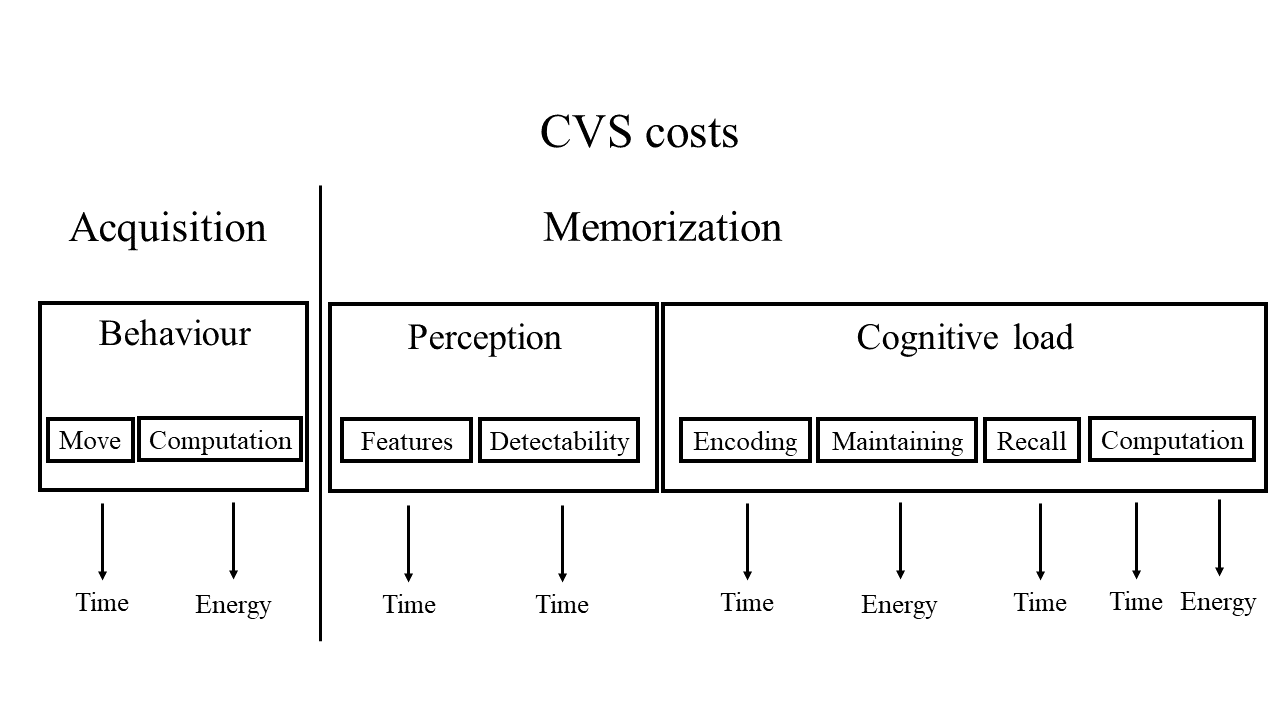
\includegraphics[width=\textwidth]{Figures/cvs costs.png}
    \caption[CVS costs]{Schematic of the possible costs in the comparative visual search task for both acquisition and memorization. The two behaviours consist of several subprocesses that entail costs of either time or metabolic energy. Own illustration after Alvarez and Cavanagh (2004).}
    \label{fig:cvs_costs}
\end{figure}

As depicted in Fig.\,\ref{fig:cvs_costs} the costs for the acquisition of information in both time and metabolic energy should be roughly positively correlated to the distance and thus time and computational effort of each gaze shift, while the costs for memorization in the CVS are somewhat more complex: Both the expenses for the perception (e.g. number of feature dimensions, detectability of information) and the encoding, maintenance, recall and computation of the information (=\,cognitive load) influence the overall memorization costs and determine visual working memory capacity limit \citep{alvarezCapacityVisualShortterm2004}. 
To investigate on this matter, we reverted to the CVS paradigm used by Hardiess and Mallot (2015), where subjects had to count the differences between two columns of stimuli. We tried to incorporate an even more controlled setup by using Gabor patches of four different orientations as comparators. This allowed us to better quantify the perceptional costs of memorization by testing for two different spatial frequencies. As Hardiess and Mallot, we also controllably varied the acquisitional costs by showing only one column at a time and inducing a delay in the change from one column to the other. To ensure that our chosen Gabor patches were within typical human perceptional range, we tested our contrast sensitivity for different spatial frequencies and whether it lies on the Campbell-Robson contrast sensitivity curve. 
 \newline
To validate the difference in perceptional cost of the two spatial frequencies tested, we conducted an experiment with a 4 Alternative Forced Choice (4AFC) task with each subject, displaying the Gabor patches for different short time frames. Findings on the influence of spatial frequency on manual reaction time \citep{breitmeyerSimpleReactionTime1975} and on saccadic reaction time \citep{ludwig2004influence}, revealed different latencies in the response of low-spatial transient and high-spatial sustained channels \citep{breitmeyerSimpleReactionTime1975}. Murray and Plainis (2003) found that the contrast gain diminishes with increasing spatial frequency and argued for the distinct gain properties of the Magnocellular (M) and Parvocellular (P) pathways as a possible neural substrate: The M channel has a high contrast gain that saturates at low contrast levels, while the P channel is much less sensitive, though within a much wider range \citep{kaplan1990new}. Consequently, the faster M channel would be responsible for target detection in typical situations, with the slower P channel only contributing at spatial frequencies over 7 cycles per degree \citep{murrayContrastCodingMagno2003}. Additional findings from \citep{chenSpatialFrequencySensitivity2018} support this theoretical framework on a level more immediate to behaviour: In the macaque brain, the superior colliculus (SC), the "saccade command center", over-represents low spatial frequencies at a population level. Accordingly, we expected that the increase in processing time for higher spatial frequencies would lead to a decrease in performance in the 4AFC task. If this held true, the high spatial-frequency Gabor patch would represent higher perceptional costs and thus lead to a change in strategy during the CVS, namingly a higher involvement of acquisition behaviour. 
 \newline
Finally, we performed an experiment on the relation of spatial frequency and contrast sensitivity in target detection.

